%----------------------------------------------------------------------------------------
%	ARTICLE CONTENTS
%----------------------------------------------------------------------------------------

\section{Introduction}

  Le surpoids et l'obésité se définissent comme une accumulation anormale ou
  excessive de graisse corporelle qui représente un risque pour la santé.

  Le surpoids et l'obésité sont des facteurs de risque majeurs pour un certain
  nombre de maladies chroniques, parmi lesquelles le diabète, les maladie
  cardio-vasculaires et le cancer. \cite{OMS}

  Pour endiguer ce mal, l'utilisation des nouvelles technologies à des fins
  éducationnelles est une voie prometteuse.

  \subsection{Contexte}

  L'agence santé publique France a lancé un appel à projets pour trouver des
  idées innovantes d'applications en lien avec l'alimentation. Nous répondons
  donc à cet appel à projets avec une idée d'application pour smartphone,
  permettant sur base des informations nutritionnelles de proposer des
  produits équivalents à ceux désirés par le consommateur mais avec de meilleurs
  propriétés nutritionnelles.

  Dans un second temps, il sera envisable d'implémenter un moteur de recommandation
  sur base des habitudes de consommation des utilisateurs de l'application.
%------------------------------------------------

\section{Objectifs}

L'objectif principal est d'étudier la faisabilité d'une telle application. Pour
ce faire, une analyse minitieuse des données contenues dans la base de données
d'openfoodfacts est nécessaire. Il s'agit dans un premier temps de cerner les
variables nécessaires au fonctionnement de l'application et ensuite vérifier
que les données permettent bien de répondre à la problématique.

\section{Problématique}

La problématique est double :\newline
La première chose est de s'assurer que les données dont on dispose contiennent
bien les informations nécessaires pour créer une telle application.\newline
La deuxième chose :\newline
Peut-on trouver dans la base de données, un produit équivalent avec
de meilleurs propriétés nutritionnelles à partir d'un produit scanné dans
un magasin?

\section{Démarche}

  Pour répondre à la problématique, on se base sur la base de données
  d'openfoodfacts (à l'heure actuelle la plus grosse base de produits alimentaire).
  Une fois les données téléchargées, ces dernières subissent un nettoyage.
  On réalise alors une analyse statistique descriptive
  sur une sélection de variables d'intérêt.
  L'analyse statistique est divisée en deux parties, les analyses univariées et
  les analyses bivariées.

  \subsection{Outils}

    \subsubsection{Matériel}

    L'analyse a été réalisée sur un ordinateur personnel
    (processeur intel i7 4 coeurs, 16 Go de RAM.) et ne nécessite pas de
    matériel particulier.

    \subsubsection{Logiciels}

    L'analyse a été réalisée avec le language Python et des notebooks Jupyter
    sont disponibles dans le répertoire Github (voir section ~\ref{Liens})

\section{Les données utilisées}

  \subsection{Généralités}

  Les données utilisées sont disponibles gratuitement auprès d'Openfoodfacts et
  sont publiées sous licence "Open Database License".

  Les données sont entrées par les utilisateurs (Applications mobiles :
  Openfoodfacts et Yuka). Par conséquent les données sont régulièrement mal
  complétées ou erronées.
  La base de données pèse actuellement (2.2 Go), elle contient (à l'heure
  actuelle\footnote{23 janvier 2020}) 1 120 752\footnote{626 672 pour les pays
  francophones (France, Suisse, Belgique et Luxembourg)} d'entrées et 178 colonnes.

  \subsection{Contenu de la base de données}

  Les champs sont séparés en quatres sections:
  \begin{itemize}
    \item Les informations générales sur la fiche du produit: nom, marque, date de création...
    \item Un ensemble de tags: catégorie du produit, localisation, origine, etc.
    \item La liste des ingrédients et les additifs éventuels.
    \item Des informations nutritionnelles: quantités au 100g (graisse, sucre, etc.).
  \end{itemize}

  \subsection{Nettoyage de la base de données}

    \subsubsection{Données concernant la France}
    On ne récupère que les données pour la France et les pays limitrophes
    francophones.

    \subsection{Variables sélectionnées}
    Pour assurer la faisabilité du projet, nous avons besoins de :
    \begin{itemize}
      \item Le nom du produit
      \item Le code bar du produit
      \item La marque du produit
      \item La catégorie à la quelle appartient le produit
      \item Le nutriscore (nutrition grade [A, ..., E])
      \item Certaines données nutritionnelles :
      \begin{itemize}
        \item Valeur énergétique au 100g
        \item Teneur en protéines
        \item Teneur en sucres
        \item Teneur en graisses
        \item Teneur en sel
      \end{itemize}
    \end{itemize}

    \subsection{Taux de remplissage des champs}

    On peut regarder le taux de remplissage des champs de manière graphique à
    l'aide d'un graphique type matrice. (chaque valeur est alors représentée
    par un tiret (les colonnes noires sont alors totalement complètes et les
    colonnes vides sont blanches.) Voir graphique \ref{completness}

    \begin{figure}[H]
      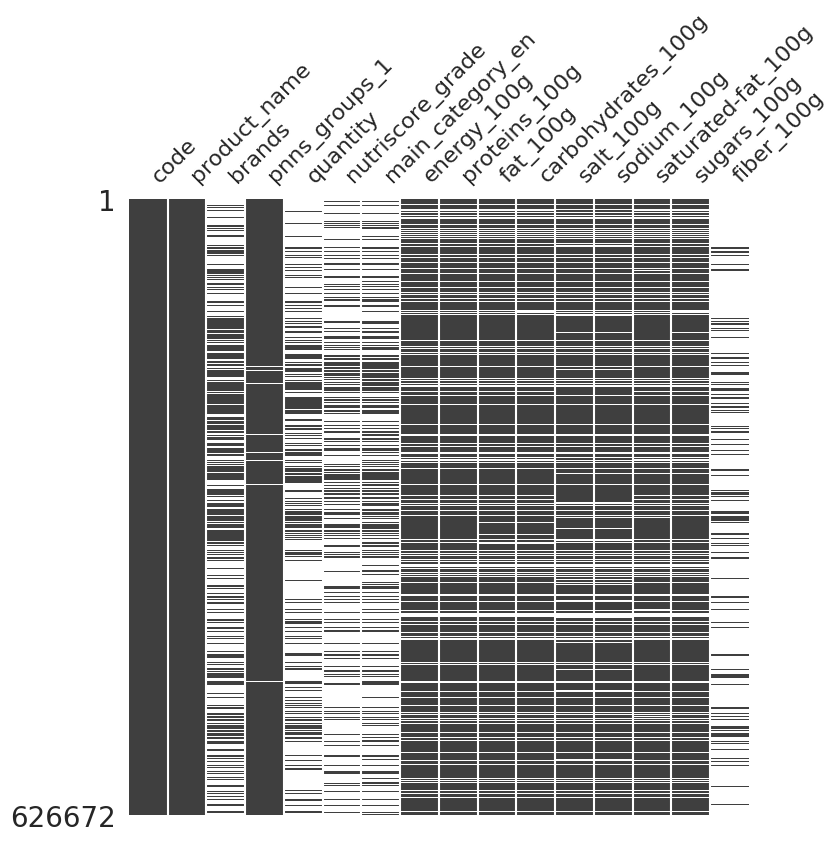
\includegraphics[width=80mm]{completness.png}
      \caption{Taux de remplissage des champs}
      \label{completness}
    \end{figure}

      \subsubsection{Stratégie appliquée aux valeurs manquantes}

      Pour les champs : \emph{quantité, nutriscore, catégorie, valeur énergétique}, on
      supprime le produit si l'une des information est manquante.

      Les champs \emph{marque, groupe PNNS 1 et 2}, on
      remplace les valeurs manquantes par une catégorie inconnue \verb|unknown|


    \subsection{Champs contenant des valeurs textuelles}

    Les champs <<PNNS groups>> <<Catégorie>> et <<Marques>> sont traités par
    méthode de <<clustering>>. L'algorithme utilisé est l'algorithme de
    <<Key collision>> méthode par défaut d'OpenRefine\cite{OpenRefine}.

    Le champs quantité est traité grace à un parser.

    \subsection{Champs numériques}

    Les champs numériques représentant une quantité de nutriments au 100g (ex : protéines)
    doivent être bornés dans l'interval $\mathbb{R}\in [0, 100]$

    Le champs <<Valeur énergétique>> est borné dans l'interval $\mathbb{R}\in [0, 4000]$
    \footnote{0 étant la valeur nutritionnelle de l'eau et l'élément le plus riche
    est la graisse $\approx 3700$KJ}

    Pour les champs correspondant à une sous classe d'un nutriment (ex : glucides et sucre)
    on vérifie que le champs <<enfant>> est inférieur ou égal au champs <<parent>>

    On vérifie en dernier lieu que la somme des valeurs protéines, graisse,
    glucides, sel et fibres est inférieur à 100g


\section{Analyses univariées}


  \subsection{Répartition du nutriscore}
  \begin{figure}[H]
    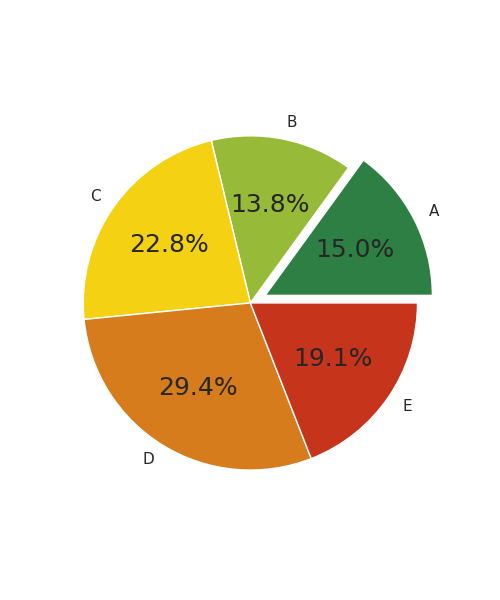
\includegraphics[width=70mm]{nutriscore_pie.png}
    \caption{Répartition du nutriscore des produits}
    \label{nutriscore_pie}
  \end{figure}
   On regarde ici la répartition des produits en fonction du nutriscore sous forme
   d'un diagramme de type camembert. On observe une répartion relativement équitable
   entre les différentes modalités. La classe D étant la plus présente et la B la moins présente.

  \subsection{Marques, groupes PNNS et catégories}
  \begin{figure}[H]
    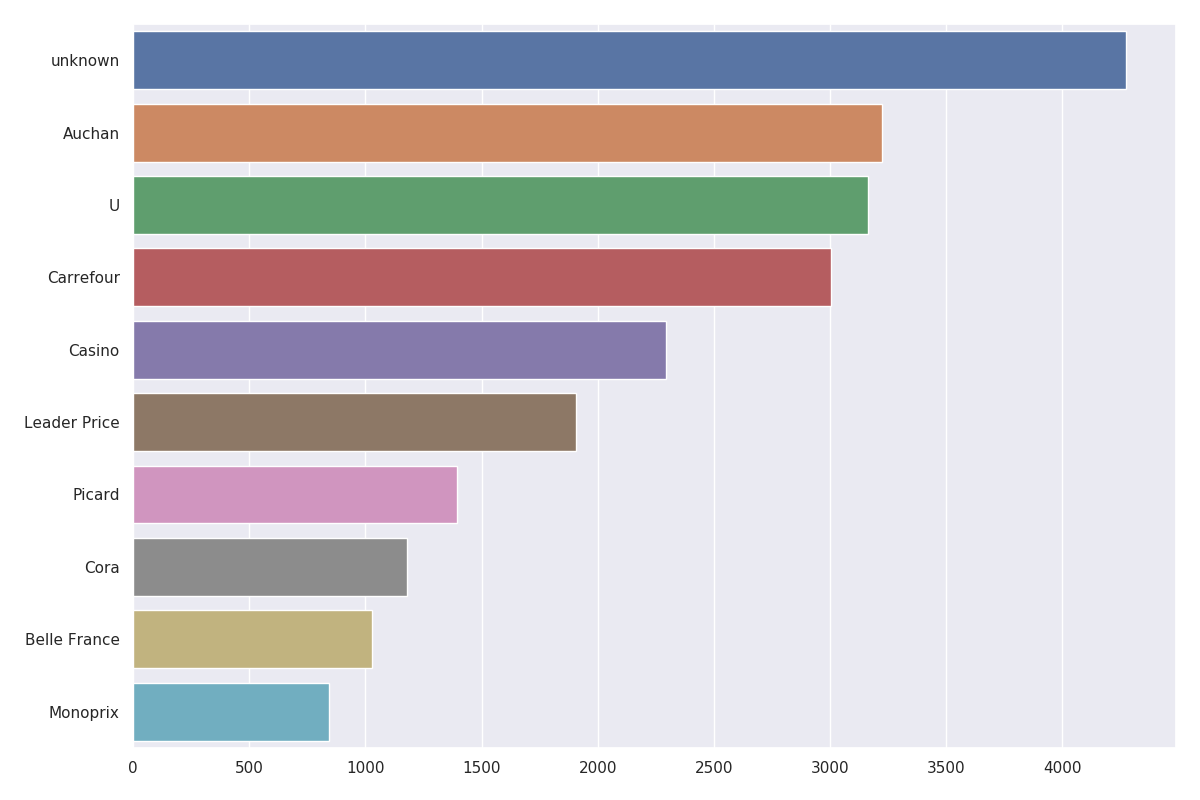
\includegraphics[width=75mm]{brands_repartition.png}
    \caption{Répartion des produits en fonction des marques}
    \label{}
  \end{figure}
  \begin{figure}[H]
    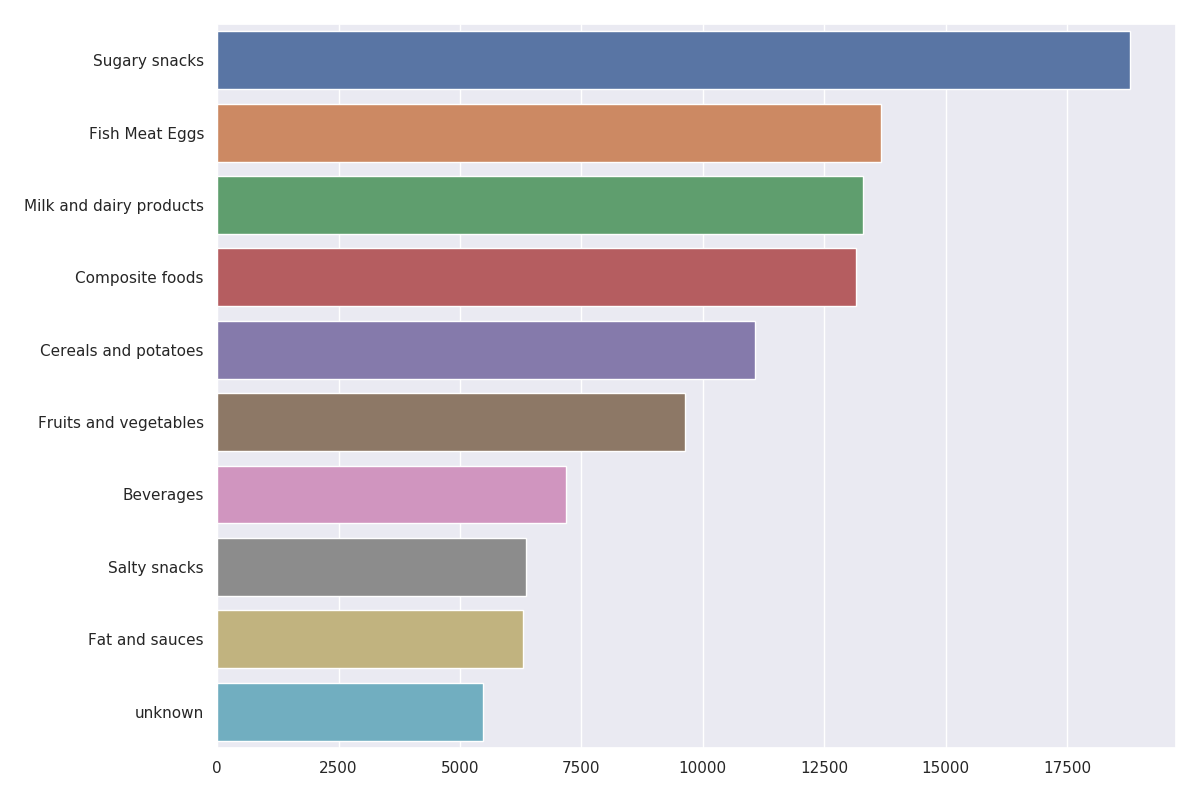
\includegraphics[width=75mm]{pnns_1_repartition.png}
    \caption{Répartion des produits en fonction du groupe PNNS}
    \label{}
  \end{figure}

  On observe qu'un grand nombre de produits n'ont pas de marque renseignée ("Unknow")
  Le graphique montre les 10 modalités les plus représentées. Cependant, il y a
  16 185 modalités présentent (dont 9572 orphelines)

  \subsection{Catégories}
  2107 modalités présentent dont 1754 orphelines. Voir \textsc{\bf{Figure \ref{wc_cat}}}
  \begin{figure*}
    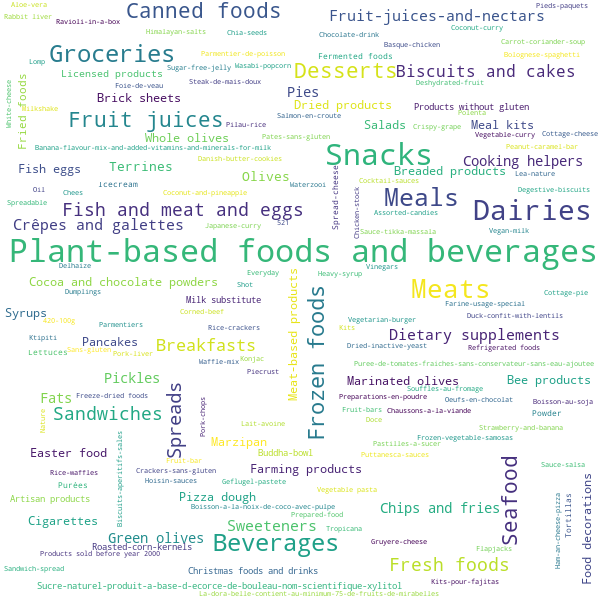
\includegraphics[width=\linewidth]{wc_categories.png}
    \caption{Les catégories présentent dans la base de données sous forme de
    nuage de mot (wordcloud)}
    \label{wc_cat}
  \end{figure*}


  \subsection{Valeurs énergétiques des produits}
  \begin{figure}[H]
    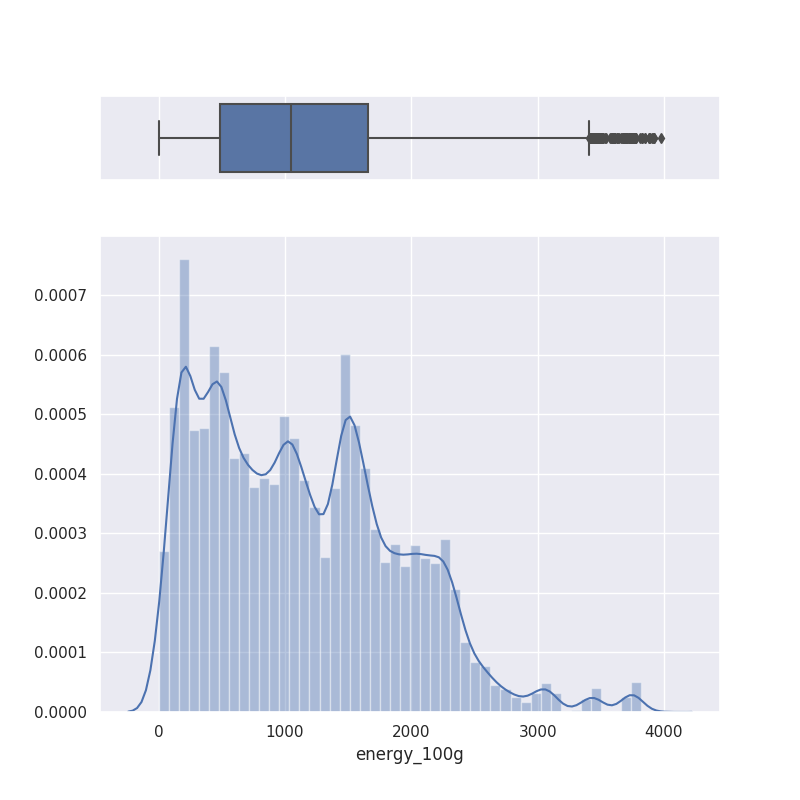
\includegraphics[width=75mm]{energy_100g-dist.png}
    \caption{Distribution des valeurs énergétiques des produits dans la base
    de données.}
    \label{}
  \end{figure}

  \subsection{Nutriments aux 100g}
  \begin{figure}[H]
    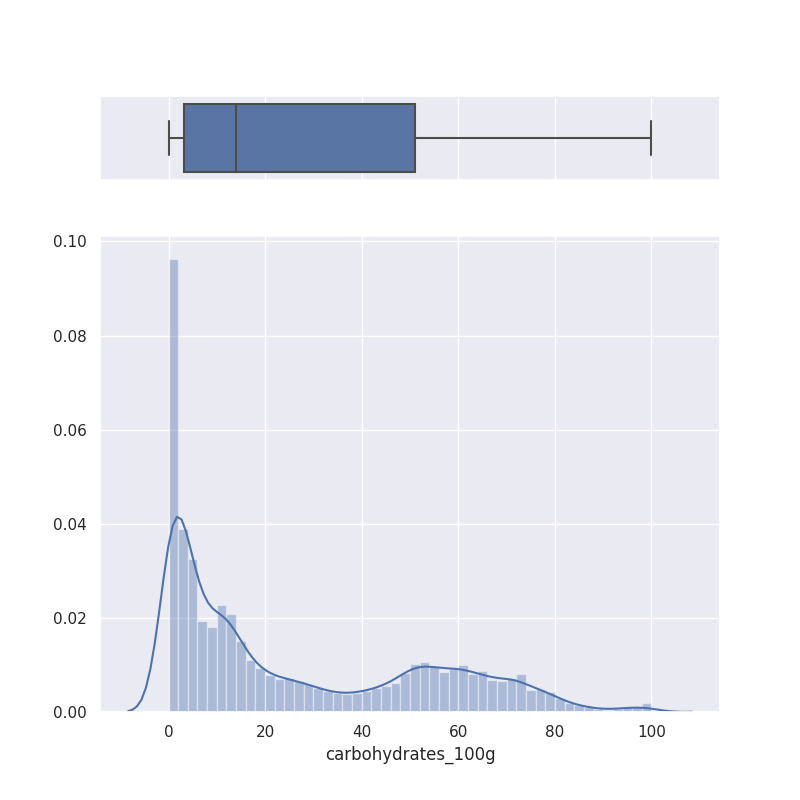
\includegraphics[width=75mm]{carbohydrates_100g-dist.png}
    \caption{Distribution de la quantité de glucides aux 100g}
    \label{}
  \end{figure}

  \begin{figure}[H]
    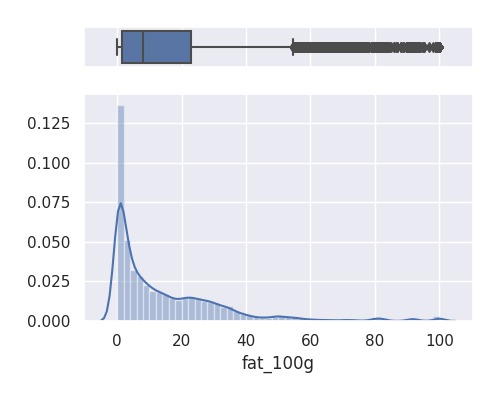
\includegraphics[width=75mm]{fat_100g-dist.png}
    \caption{Distribution de la quantité de graisse aux 100g}
    \label{}
  \end{figure}
  \begin{figure}[H]
    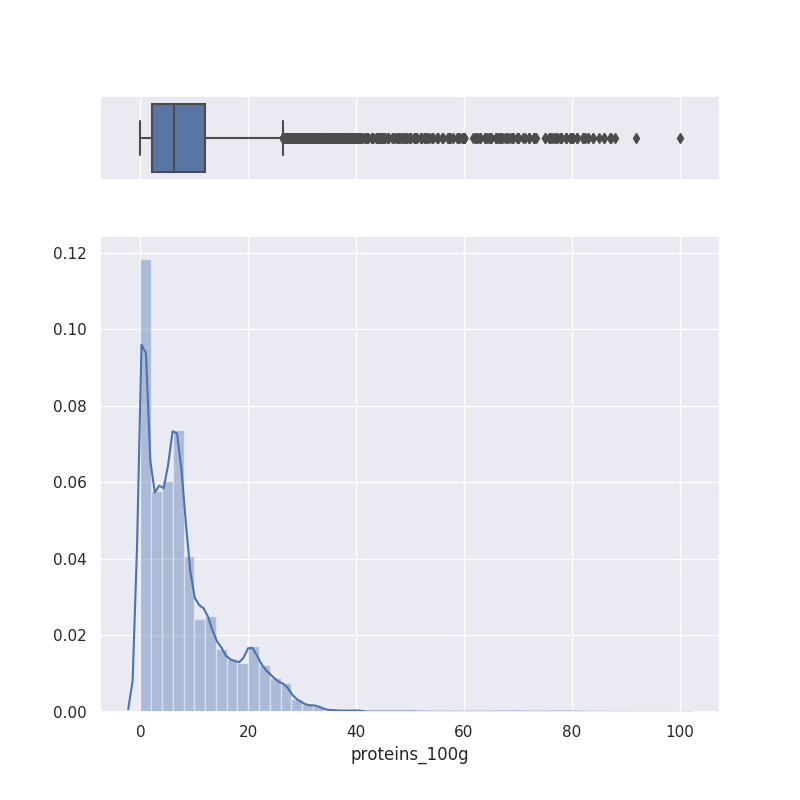
\includegraphics[width=75mm]{proteins_100g-dist.png}
    \caption{Distribution de la quantité de protéines aux 100g}
    \label{}
  \end{figure}


\section{Analyses multivariées}
Toujours dans l'objectif de trouver un produit équivalent, il est important
de vérifier que pour chaque catégorie (ici groupe Programme national nutrition santé PNNS)
il existe des produits pour chaque nutriscore (de A à E).

  \subsection{Nutriscore et marques}
    \begin{figure}[H]
      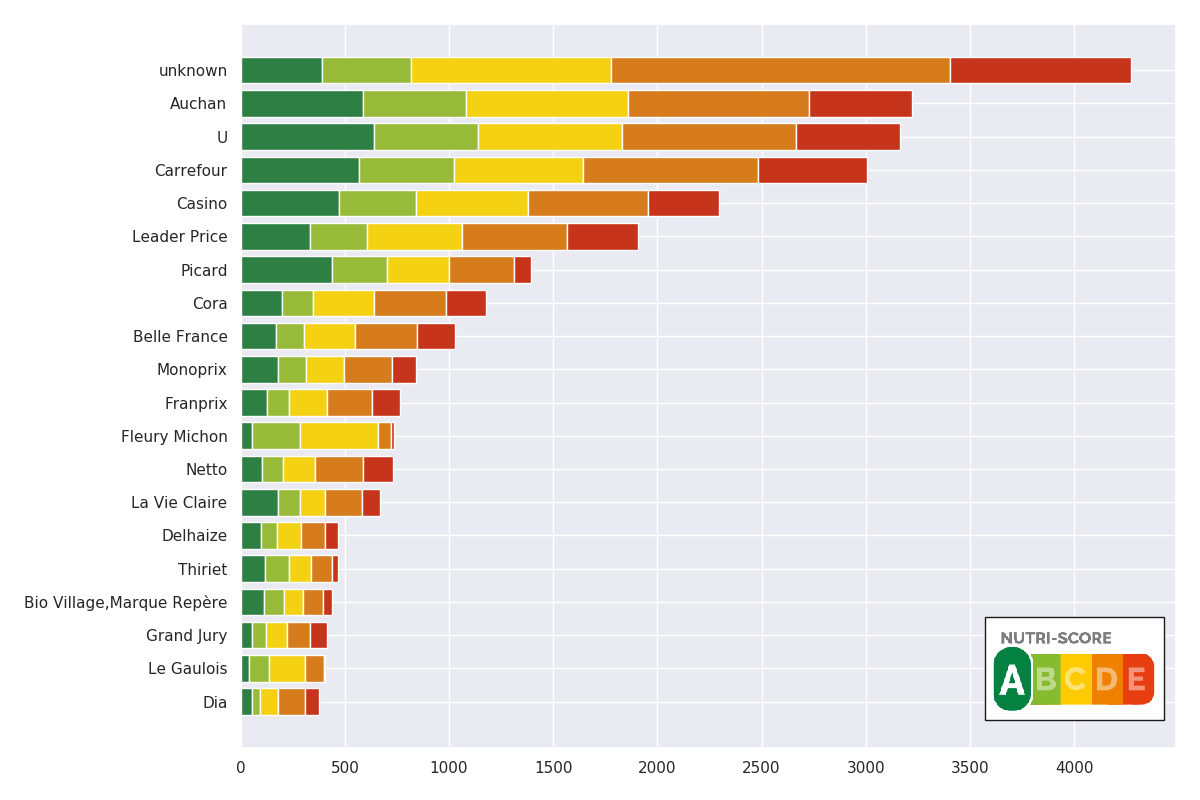
\includegraphics[width=75mm]{brands_nutscore_repartition.png}
      \caption{Repartition du nutriscore au sein des marques}
      \label{}
    \end{figure}
    \begin{figure}[H]
      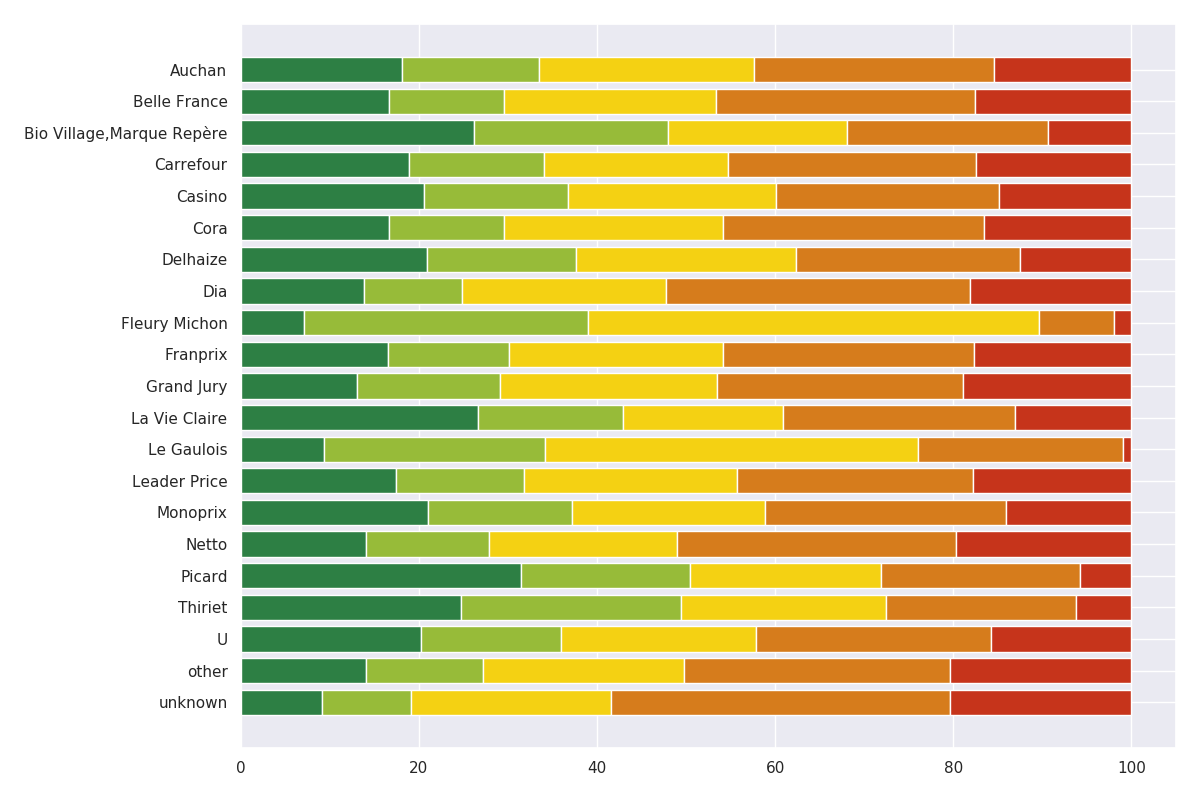
\includegraphics[width=75mm]{brands_nutscore_repartition_freq.png}
      \caption{Repartition du nutriscore au sein des marques (normalisé en fréquence)}
      \label{}
    \end{figure}

  \subsection{Nutriscore et groupes PNNS}
  \begin{figure}[H]
    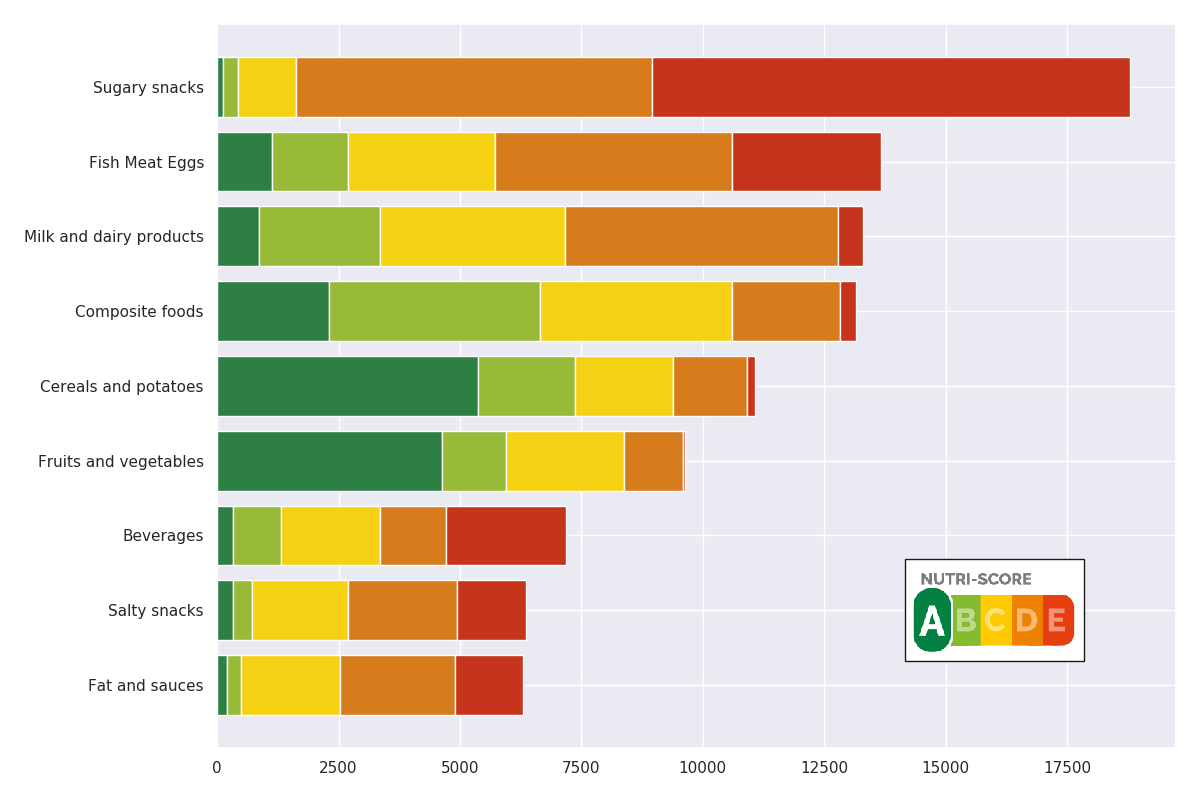
\includegraphics[width=75mm]{pnns1_nutscore_repartition.png}
    \caption{Repartition du nutriscore au sein des groupes PNNS}
    \label{}
  \end{figure}
  \begin{figure}[H]
    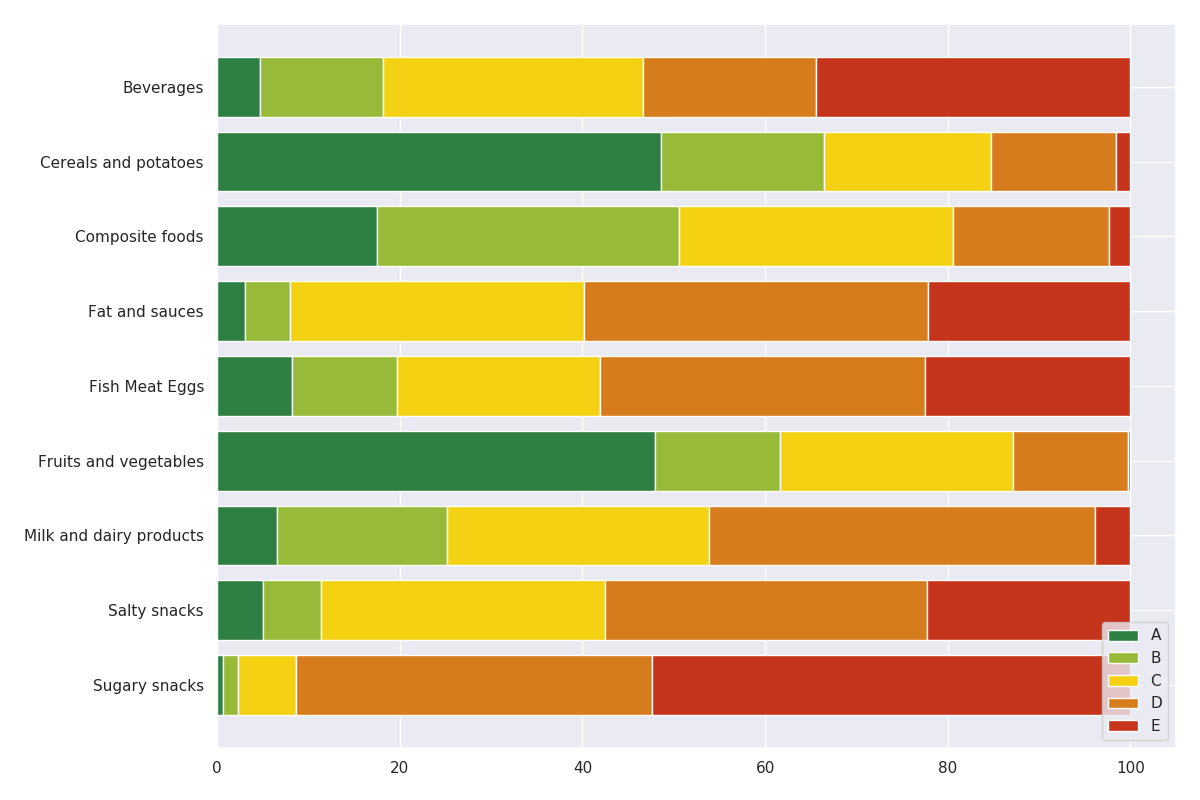
\includegraphics[width=75mm]{pnns1_nutscore_repartition_freq.png}
    \caption{Repartition du nutriscore au sein des groupes PNNS (normalisé en fréquence)}
    \label{}
  \end{figure}

  \begin{table}[H]
    \footnotesize\setlength{\tabcolsep}{2.5pt}
    \caption{Tableau de contingence groupe PNNS et Nutriscore}
    \label{}
    \begin{tabular}{lrrrrr}
\toprule
nutriscore\_grade &      a &      b &      c &      d &      e \\
pnns\_groups\_1           &        &        &        &        &        \\
\midrule
Beverages               &    335 &    972 &   2038 &   1359 &   2473 \\
Cereals and potatoes    &   5375 &   1984 &   2022 &   1520 &    168 \\
Composite foods         &   2303 &   4347 &   3946 &   2239 &    311 \\
Fat and sauces          &    192 &    308 &   2028 &   2367 &   1393 \\
Fish Meat Eggs          &   1121 &   1564 &   3041 &   4874 &   3071 \\
Fruits and vegetables   &   4621 &   1317 &   2449 &   1215 &     27 \\
Milk and dairy products &    871 &   2478 &   3814 &   5615 &    517 \\
Salty snacks            &    319 &    401 &   1981 &   2239 &   1412 \\
Sugary snacks           &    116 &    322 &   1181 &   7337 &   9848 \\
unknown                 &    487 &    737 &   1431 &   2029 &    782 \\
Sum                     &  15740 &  14430 &  23931 &  30794 &  20002 \\
\bottomrule
\end{tabular}

  \end{table}

  \subsection{Valeurs énergétiques des aliments et nutriscore}
  \begin{figure}
    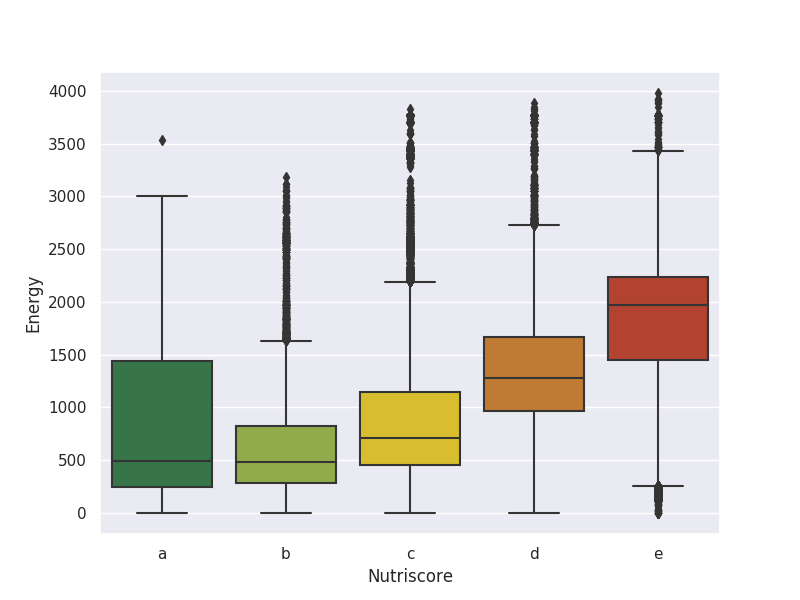
\includegraphics[width=90mm]{box_plot_energy_nutscore.png}
    \caption{}
    \label{}
  \end{figure}

  \subsection{Nutriscore / valeurs énergétiques / composition des produits}


  \begin{figure*}[h]
    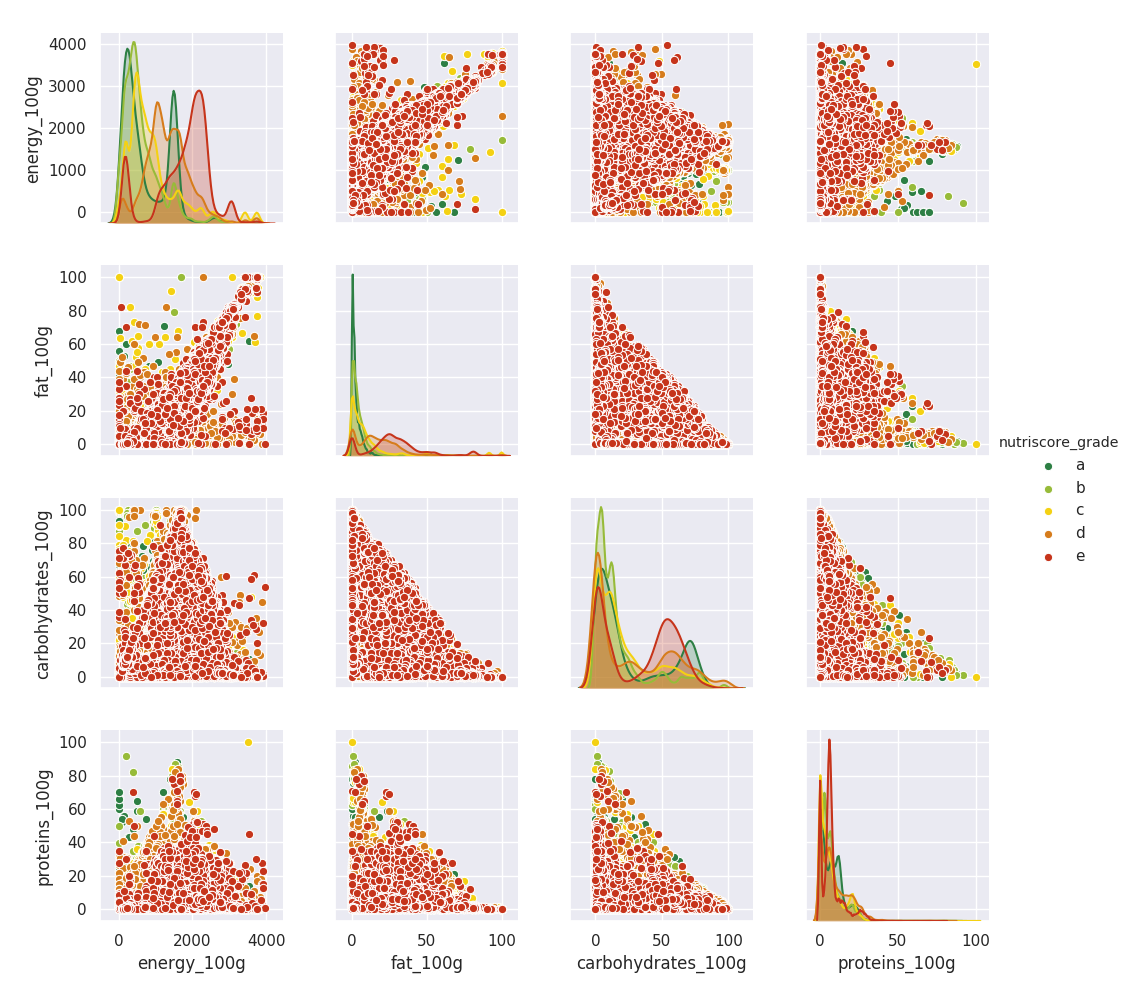
\includegraphics[width=\linewidth]{relational_plot.png}
    \caption{}
    \label{relplot}
  \end{figure*}

  voir \textsc{\bf{Figure \ref{relplot}}}
\section{Conclusions}

La base de données Openfoodfacts est une bonne base, cependant cette dernière
demande un travail complexe de traitement. A l'heure actuelle, il est possible
de rechercher des produits équivalents au sein du même groupe PNNS 1, d'affiner
(dégrossir) la recherche sur base du groupe PNNS 2 et finalement affiner les
résultats sur base de la catégorie.

Prenons un exemple simple, l'utilisateur scan un steack haché au rayon boucherie,

\section{Perspectives}

%\section*{Remerciements}

\section{Liens internet}
\label{Liens}
\begin{itemize}
  \item \faGithub \url{https://github.com/tgrandjean/OC-sante-publique-france}
  \item \faDatabase \url{https://world.openfoodfacts.org/data}
  \item \faFileO \url{https://tgrandjean-oc-reports.s3.eu-west-3.amazonaws.com/openfoodfacts/profiling_report.html}
\end{itemize}
